% !TeX spellcheck = it_IT
\documentclass[a4paper,12pt]{article}

\usepackage{alltt, fancyvrb, url}
\usepackage{graphicx}
\usepackage{algorithmic}
\usepackage[utf8]{inputenc}
\usepackage{titling}
\usepackage{fancyhdr}
\usepackage{fontenc}
\usepackage{amsmath,mathtools,algorithm}
\usepackage{amssymb}
\usepackage{longtable}
\usepackage{setspace}
\usepackage{listings}
\usepackage{color}
\usepackage{eurosym}
\usepackage{array}
\usepackage[referable]{threeparttablex}
\usepackage{pifont}

\newcommand{\cmark}{\ding{51}}
\newcommand{\xmark}{\ding{55}}

\usepackage[italian,hidelinks]{hyperref}

\usepackage[italian]{babel}
\usepackage[italian]{cleveref}


\pretitle{%
	\begin{center}
		\LARGE
	}
\posttitle{\end{center}}


\title{\Huge \textbf{Briscola Simulation} \\
	\vspace{10pt}
	\vspace{20pt}
}
\author{
	Gabriele Graffieti \\ \small \url{gabriele.graffieti@studio.unibo.it}
	\vspace{15pt}
	\\
	Alfredo Maffi \\ \small \url{alfredo.maffi@studio.unibo.it}
	\vspace{15pt}
	\\
	Manuel Peruzzi \\ \small \url{manuel.peruzzi@studio.unibo.it}
}

\date{}

\begin{document}

\maketitle
\pagenumbering{arabic}
\newpage
\tableofcontents
\newpage
\section{Introduzione}

Questo documento è la relazione del progetto Briscola Simulation, realizzato per il corso di Sistemi Autonomi, erogato dalla facoltà di Ingegneria e Scienze Informatiche dell'Università di Bologna (A.A. 2017/2018). L'obiettivo del progetto è lo sviluppo di un sistema autonomo nel quale sia possibile simulare una partita di briscola a quattro giocatori. Questa relazione non si limita alla documentazione del software, ma deve essere vista come una descrizione dell'intero processo di sviluppo che ha portato alla realizzazione dello stesso.

Il processo di sviluppo adottato ha seguito una filosofia \emph{top-down}: è presente una prima fase di raccolta e analisi dei requisiti, seguita dalle fasi di analisi del problema e studio di fattibilità, nelle quali sono state esaminate le principali problematiche proponendo possibili soluzioni. Si passa poi ad una fase di progettazione, nella quale vengono definiti architettura del sistema e design di dettaglio dei singoli componenti. Infine, vengono stabilite le tecnologie da utilizzare per procedere poi all'implementazione del software.

\section{Analisi dei requisiti} \label{requirements-analysis}

In questo sezione verranno elencati ed analizzati i requisiti del sistema da realizzare. 

\subsection{Requisiti}

Lo scopo del progetto è quello di realizzare un sistema software in grado di simulare una partita di briscola a quattro giocatori. I giocatori dovranno sottostare al regolamento illustrato nella sezione \emph{\hyperref[briscola-rules]{regole del gioco}} fornita in appendice. Ognuno di essi dovrà cooperare con il proprio compagno al meglio delle proprie capacità per poter vincere la partita. Più nel dettaglio, i requisiti sono i seguenti:
\begin{itemize}
	\item Le squadre devono essere scelte a caso, così come il primo giocatore ad inizio partita.
	\item Le carte del mazzo devono essere distribuite da un mazziere, seguendo l'ordine indicato nelle \emph{\hyperref[briscola-rules]{regole del gioco}} in appendice. Il mazziere, mano dopo mano, distribuirà le carte fino all'esaurimento del mazzo.
	\item Un giocatore può iniziare a parlare con il compagno solamente quando è di mano ed è il primo della propria squadra a giocare per la mano corrente. Fa eccezione la prima mano, in cui non è consentito parlare.
	\item Quando un giocatore parla, tutti gli altri devono essere in grado di sentirlo. Inoltre, il compagno è sempre tenuto a rispondere.  Non sono ammessi \emph{bluff}: ogni giocatore, quando parla o risponde, è sempre obbligato a dire la verità.
	\item Ogni giocatore deve avere come obiettivo quello di massimizzare il punteggio della propria squadra, e non quello individuale.
	\item Ogni giocatore determina la propria giocata seguendo un propria logica interna, facendo affidamento su informazioni di varia natura. Tali informazioni sono costituite da:
	\begin{itemize}
		\item L'insieme delle carte che ha in mano.
		\item Eventuali carte giocate sul tavolo da gioco dagli altri giocatori in questa mano.
		\item Ciò che è stato detto dagli altri giocatori in questa mano.
		\item Le carte giocate nell'ultima presa, che saranno reperibili sul tavolo da gioco.
		\item Opzionalmente, le carte giocate nelle prese precedenti all'ultima.
		\item Opzionalmente, ciò che è stato detto dagli altri giocatori in precedenza.
	\end{itemize}
\end{itemize}

\subsection{Glossario} \label{glossary}

\begin{description}
	\item[Mazzo]: insieme di 40 carte disposte a pila in ordine casuale. Ogni carta è caratterizzata da un valore ed un seme. I valori sono 10: comprendono i numeri da 1 a 7 e le figure \emph{fante}, \emph{cavallo} e \emph{re}. I semi sono 4: denari, bastoni, spade e coppe.
	\item[Mazziere]: entità separata dai giocatori, avente l'unico scopo di distribuire le carte del mazzo ai giocatori stessi. 
	\item[Mano]: termine utilizzato per indicare un turno completo di gioco, in cui ogni giocatore gioca una carta a partire dal primo giocatore in senso antiorario. Il primo giocatore è colui che ha vinto l'ultima presa, ad eccezione del primo turno, dove viene scelto casualmente.
	\item[Presa]: l'insieme delle quattro carte sul tavolo al termine di una mano, che verranno assegnate al giocatore che ha calato la carta dominante. Per carta dominante s'intende quella specificata nel regolamento in appendice.
	\item[Essere di mano]: un giocatore è di mano quando tocca a lui giocare una carta.
	\item[Fascia di valore]: raggruppamento di carte sulla base del loro valore. Le fasce sono tre: \emph{carico} (3 e asso), \emph{figura} (re, cavallo e fante) e \emph{liscia} (7, 6, 5, 4, 2).
	\item[Parlare]: scambio di informazioni tra due giocatori di una squadra. Il giocatore che \emph{parla} pone una domanda al compagno, il quale deve rispondere in maniera binaria (``sì'' o ``no''). Tale domanda è finalizzata all'acquisizione di informazioni relative alle carte del compagno. Ogni domanda può contenere l'indicazione di una fascia di valore, di un seme o di entrambi: chi la riceve risponde positivamente soltanto se possiede almeno una carta conforme all'indicazione. Seguono due esempi di domande lecite:
	\begin{itemize}
		\item "Hai una \emph{figura} di \emph{bastoni}?"
		\item "Hai una carta di \emph{denari}?"
	\end{itemize} 
	Presupponendo che chi riceve la domanda abbia in mano cavallo di bastoni, quattro di coppe e due di spade, risponderà positivamente alla prima domanda e negativamente alla seconda.   
	\item[Tavolo da gioco]: astrazione del tavolo fisico sul quale viene disputata la partita di briscola. Su di esso saranno posizionate le carte della mano corrente e la presa della mano precedente.
\end{description}

\subsection{Modello del dominio} \label{domain-model}

\subsubsection{Struttura}

Dai requisiti sopra elencati, è possibile individuare sei componenti all'interno del sistema:
\begin{itemize}
	\item Quattro giocatori, divisi in coppie in due squadre.
	\item Un mazziere, responsabile della distribuzione delle carte. \'E un'entità separata che non partecipa alla partita.
	\item Un tavolo da gioco, necessario per giocare carte e tenere memoria dell'ultima presa. 
\end{itemize}

Siccome i giocatori sono entità autonome con un proprio stato interno ed una capacità di \emph{reasoning} necessaria alla scelta delle carte da giocare, viene naturale modellarli come entità attive. Allo stesso modo, pur non avendo la stessa capacità di \emph{reasoning}, anche il mazziere è modellato come entità attiva. Infine, vien naturale modellare il tavolo come un'entità passiva, finalizzata a mantenere lo stato dell'ultima mano e di quella corrente. 

\subsubsection{Comportamento}

Di seguito è illustrato lo svolgimento di una partita, in modo da mettere in evidenza il comportamento del sistema e l'interazione tra i suoi componenti. Si presuppone che le due squadre siano già state formate e che i giocatori siano disposti come da regolamento.

\begin{enumerate}
	\item Il mazziere mischia il mazzo, distribuisce 3 carte ad ogni giocatore ed infine scopre una carta, il cui seme sarà la briscola per la partita corrente.
	\item Il primo giocatore, scelto casualmente, gioca una carta calandola sul tavolo, seguito dai restanti giocatori in senso antiorario.
	\item Quando tutte le quattro carte sono sul tavolo, queste vengono attribuite al giocatore vincente, che sarà il primo giocatore della prossima mano. A questo punto il mazziere distribuisce una carta ad ogni giocatore seguendo l'ordine della mano successiva, terminando così la mano corrente.
	\item Nelle seguenti mani, si procederà allo stesso modo (passi 2 e 3), con la possibilità di parlare da parte dei primi due giocatori di mano.
	\item Si procede fino all'esaurimento delle carte del mazzo e delle carte in mano ai giocatori. A questo punto, si procede al conteggio dei punti delle due squadre. Se una squadra ha totalizzato più di 60 punti è eletta vincitrice.
\end{enumerate}

Di seguito sono riportati due diagrammi a stati dai quali è possibile evincere comportamento dei giocatori e comportamento del mazziere rispettivamente in \autoref{player-state-diagram} e in \autoref{dealer-state-diagram}.

\begin{figure}[H]
	\centering
	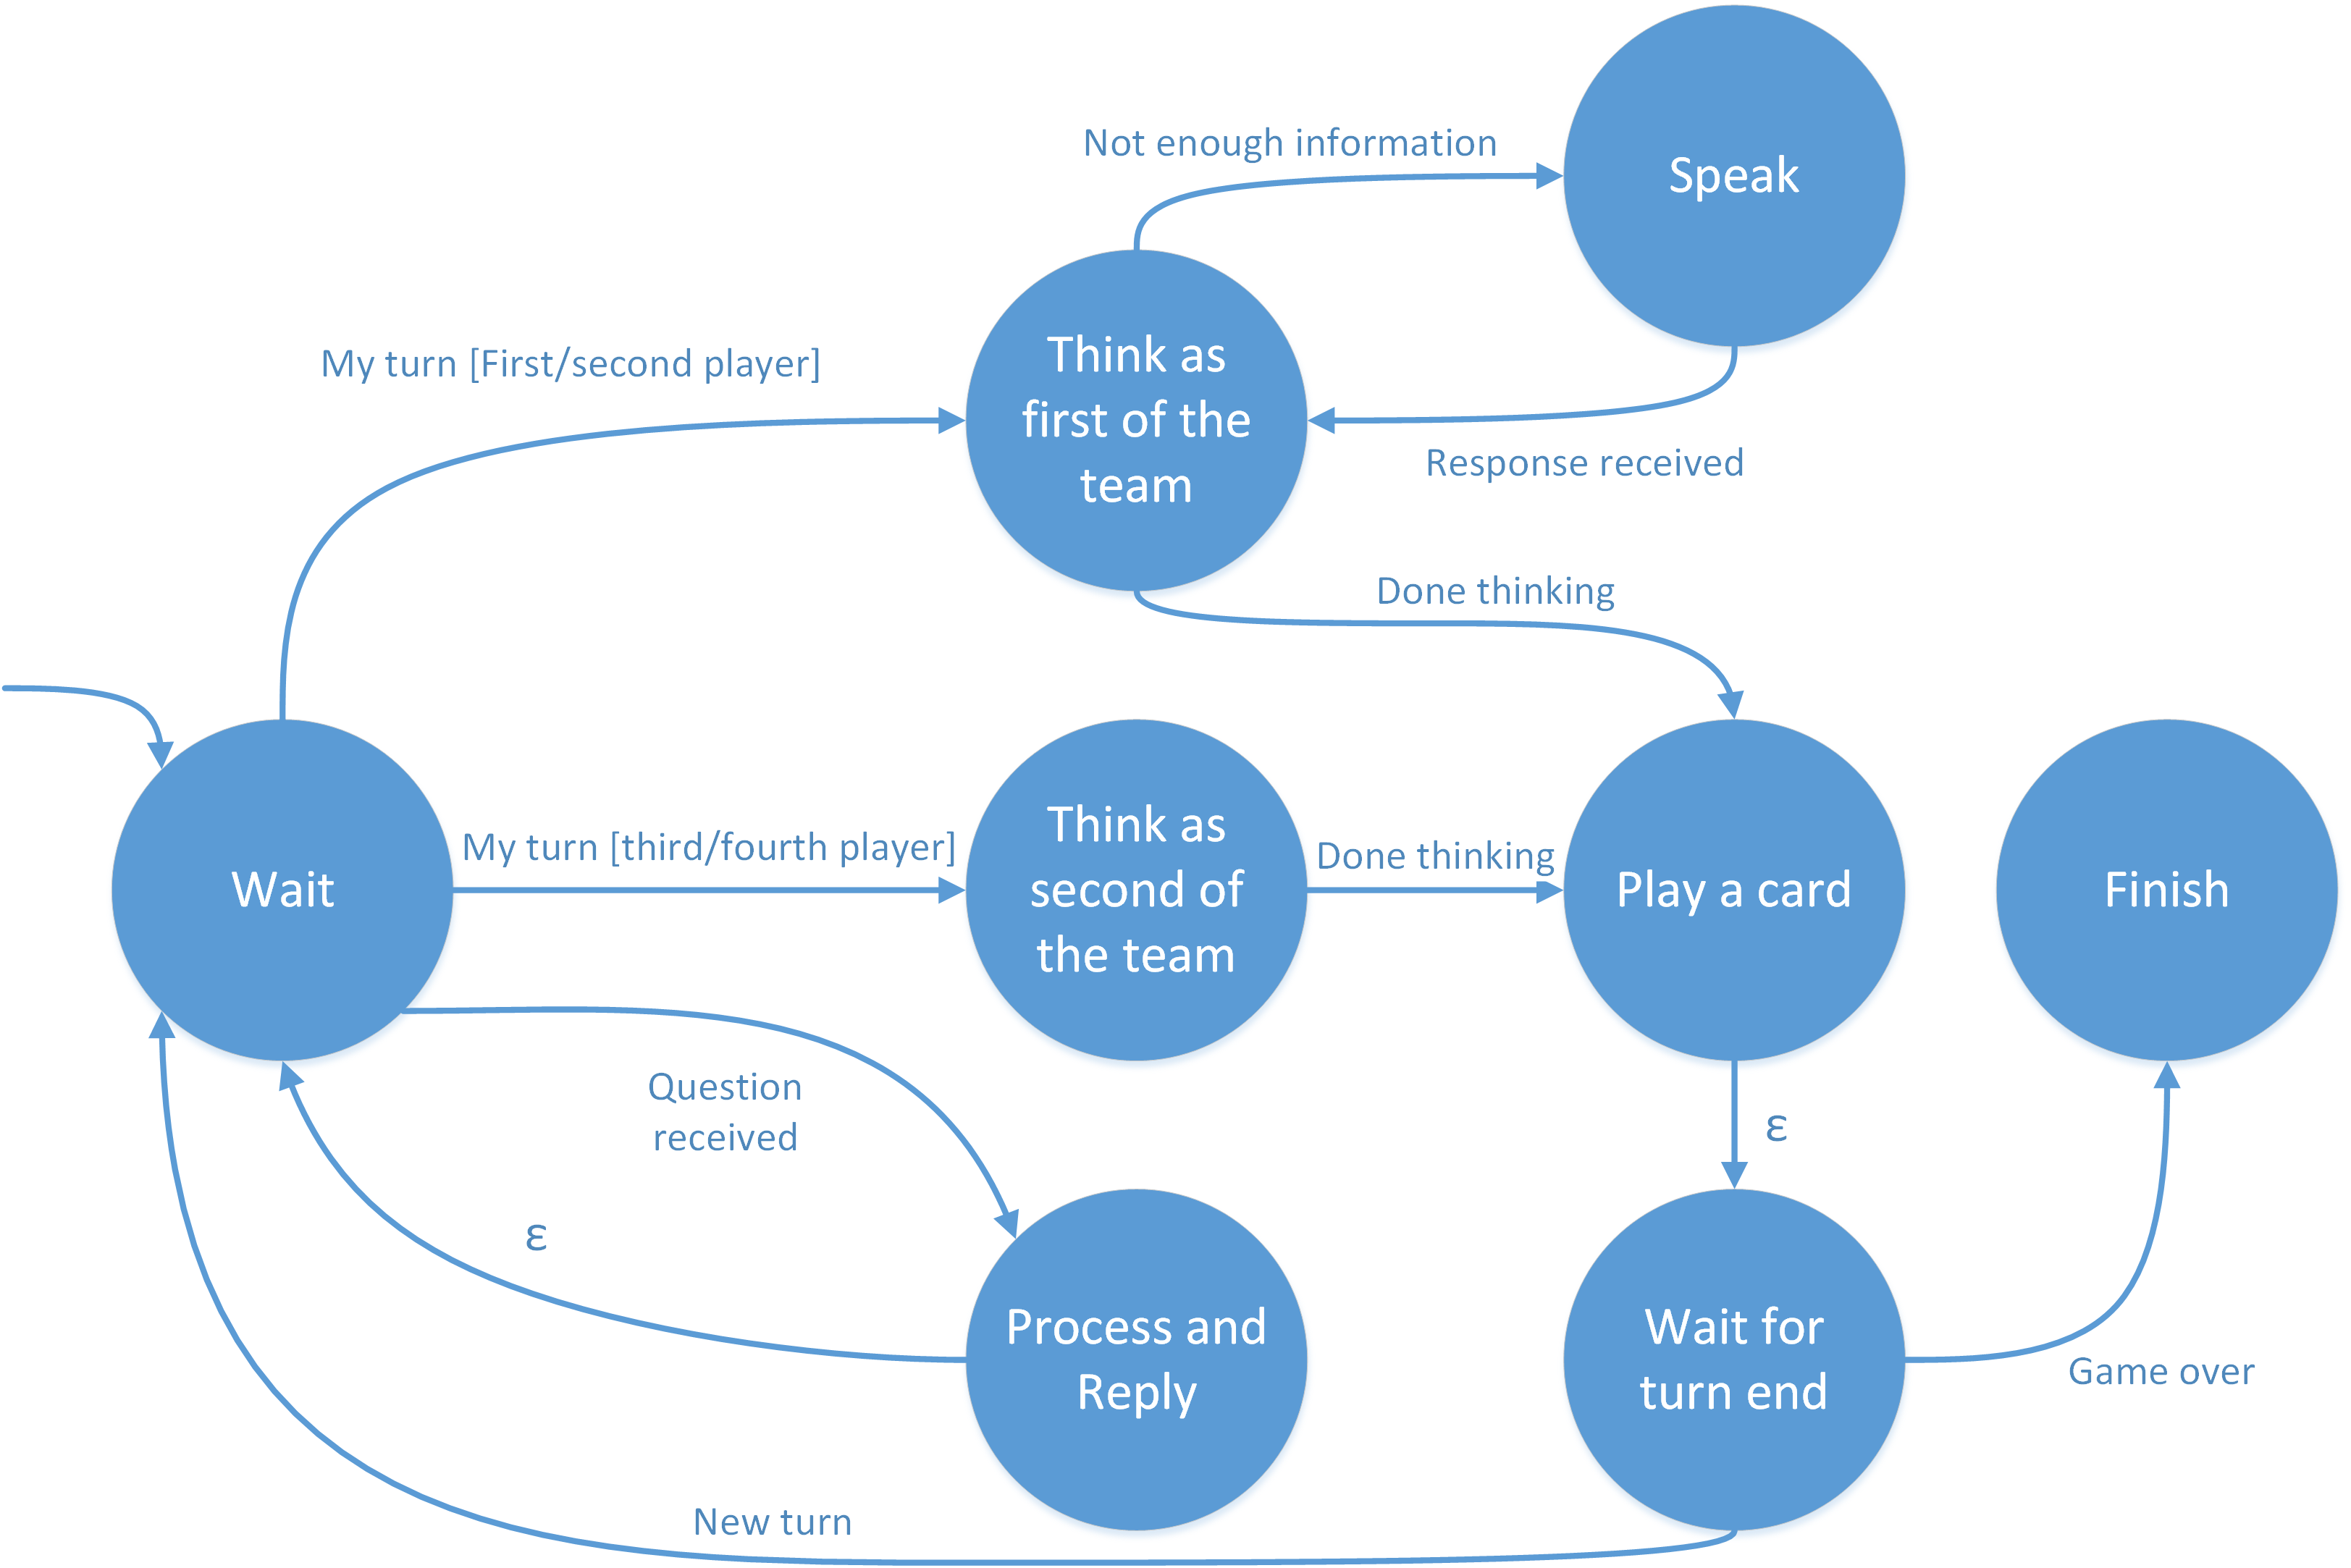
\includegraphics[width=140mm]{./img/player_state_diagram.png}
	\caption{Diagramma a stati di un giocatore.  \label{player-state-diagram}}
\end{figure}


\begin{figure}[H]
	\hspace*{-0.7in}
	\centering
	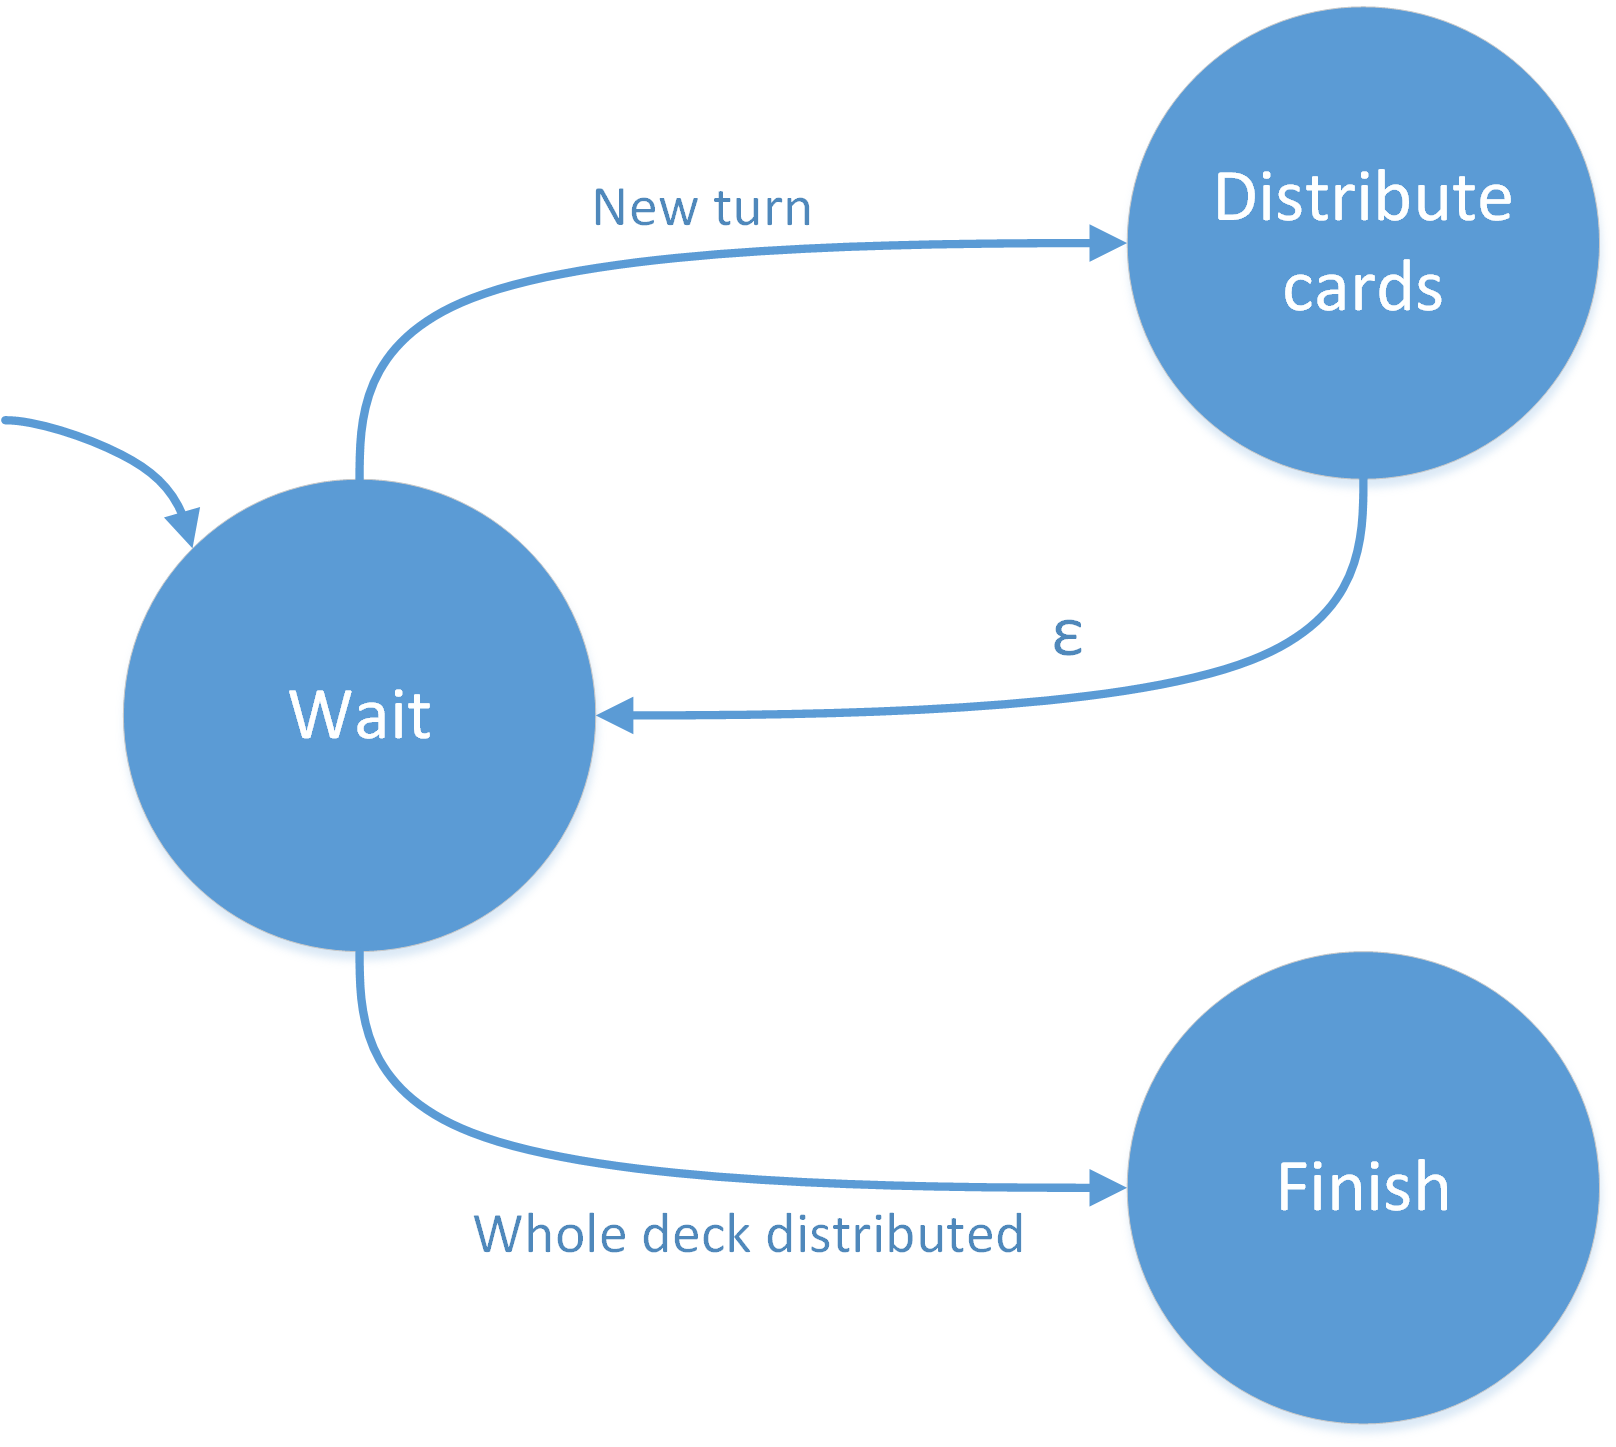
\includegraphics[width=70mm]{./img/dealer_state_diagram.png}
	\caption{Diagramma a stati del mazziere.  \label{dealer-state-diagram}}
\end{figure}

\subsubsection{Interazione}

Consultando i requisiti, è facile notare che l'interazione tra i componenti del sistema costituisce il punto focale del progetto, se non quello più delicato e complesso. Siccome dai requisiti stessi non è possibile evincere un unico schema di interazione, è necessaria un'analisi nel dettaglio per determinare lo schema migliore, effettuato nelle prossime sezioni.  

\section{Analisi del problema} \label{problem-analysis}
Il modello del dominio, individuato in \autoref{domain-model}, non risulta adeguatamente sviluppato per procedere alla fase di progettazione del sistema. I componenti individuati, infatti, non sono sufficienti per un completo svolgimento di una partita. Importanti funzionalità del sistema consistono nella creazione delle squadre, nell'assegnamento di ogni presa al giocatore vincente, nel conseguente conteggio finale dei punti accumulati dalle due squadre e nella proclamazione della squadra vincitrice. Tali funzionalità non sono ricoperte da nessuno dei componenti individuati. L'unico di essi che concettualmente potrebbe svolgere tali compiti è il tavolo da gioco. Le funzionalità espresse in precedenza implicano che il componente che ne è responsabile sia un'entità attiva con un proprio flusso di controllo. Il tavolo, modellato in precedenza come entità passiva, non risulta adeguato a svolgere tali mansioni. Perciò si rende necessaria l'introduzione di un nuovo componente, ovvero \emph{arbitro}.

Inoltre, dai requisiti non è chiaro in che modo le entità del sistema possano coordinarsi tra loro durante lo svolgimento di una partita. In particolare, non è specificata la modalità tramite la quale un giocatore sappia qual è il momento adatto per effettuare la sua giocata in una determinata mano. Allo stesso modo, non è indicato come il mazziere venga a conoscenza del momento in cui si conclude la fase di assegnazione della mano, per poi procedere alla distribuzione delle carte. Questa problematica potrebbe essere risolta in diversi modi:
\begin{itemize}
	\item \textbf{Introduzione di un orchestratore}: la coordinazione tra le entità del sistema potrebbe essere garantita dall'introduzione di un nuovo componente adibito.
	\item \textbf{Assegnamento del compito di orchestratore all'arbitro}: data la concezione di arbitro, non è difficile immaginare che possa essere proprio tale componente a fornire anche funzionalità di coordinazione di una partita.
	\item \textbf{Coordinazione tramite le informazioni sul tavolo}: siccome il tavolo è l'entità sulla quale si svolge la partita, esso potrebbe essere considerato come una sorgente di informazioni ed eventi, utilizzabili da giocatori, mazziere e arbitro per coordinarsi.
\end{itemize}
Fra le opzioni elencate, è sembrato più appropriato mettere in atto la seconda, attribuendo all'arbitro il ruolo di orchestratore della partita.

Sulla base di quanto discusso, in \autoref{general-sequence-diagram} è illustrato un diagramma di sequenza, in modo da mettere in evidenza l'interazione tra i componenti del sistema durante il primo turno di gioco.


\begin{figure}[H]
	\hspace*{-0.7in}
	\centering
	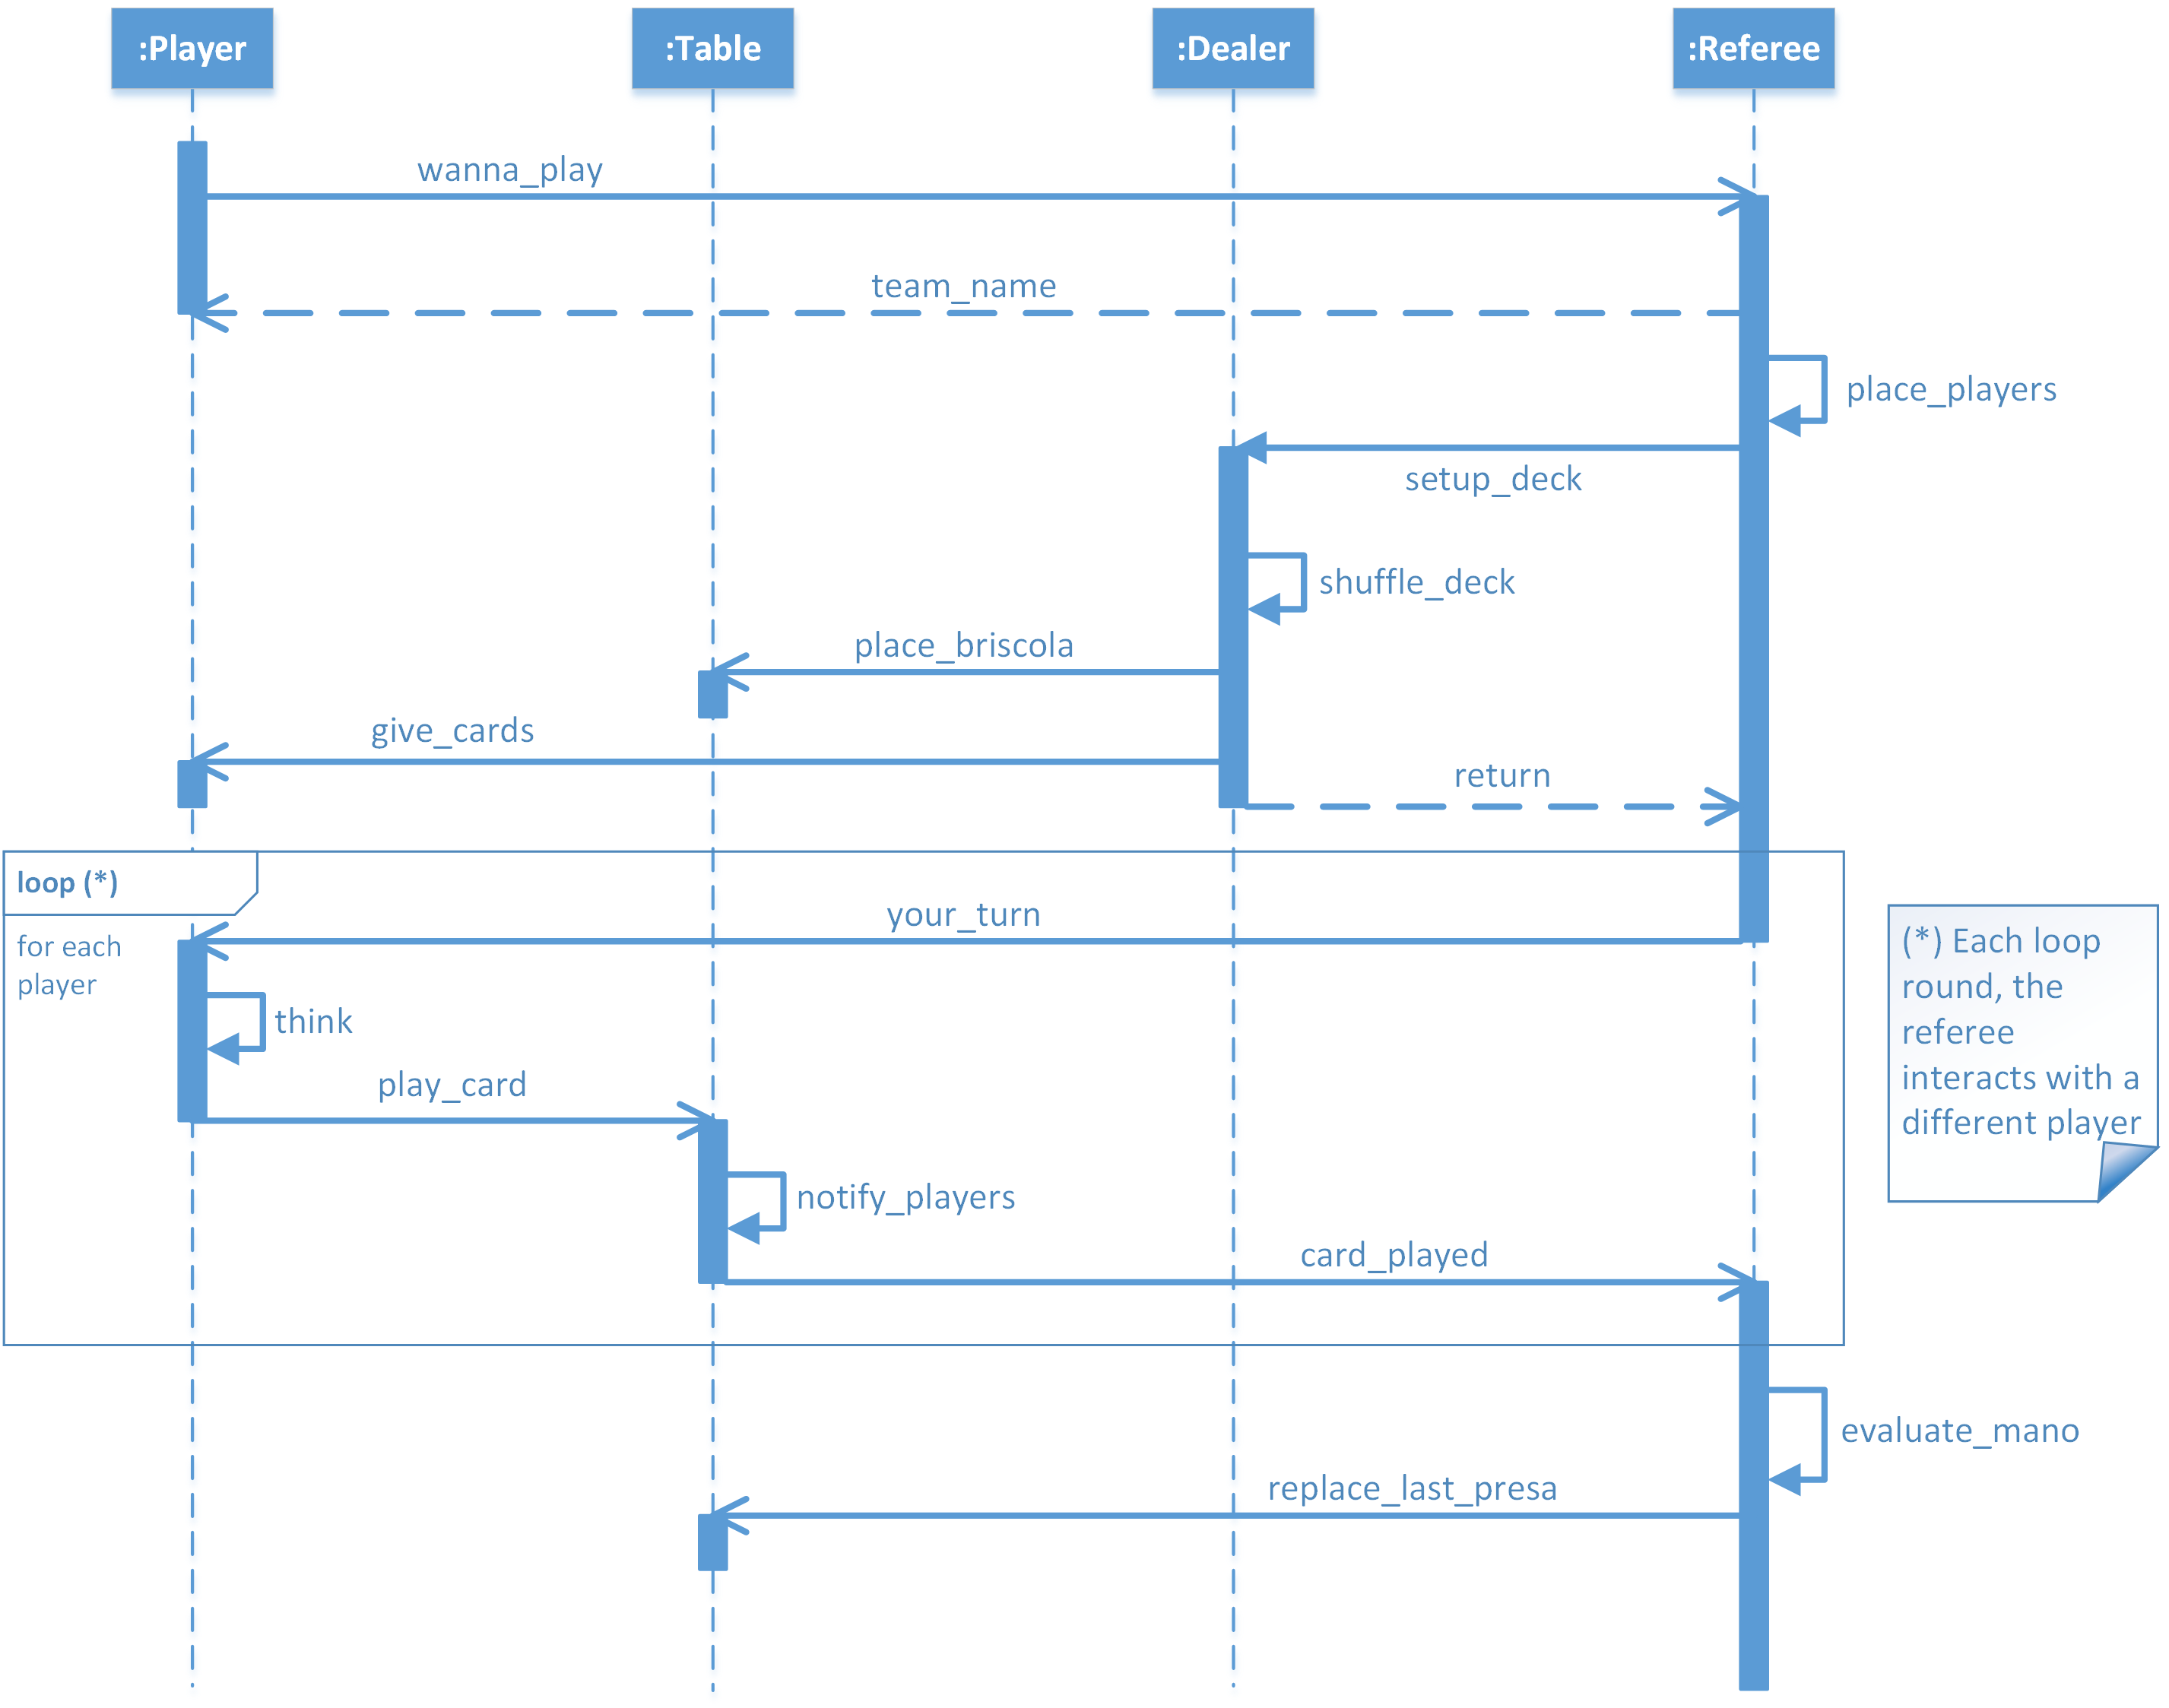
\includegraphics[width=180mm]{./img/general_sequence_diagram.png}
	\caption{Diagramma di sequenza del sistema per il primo turno. Per motivi grafici non sono stati inclusi nella rappresentazione tutti i giocatori di una partita, ma solamente uno di essi. \label{general-sequence-diagram}}
\end{figure}

Le mani successive sono molto simili alla prima, anche se presentano una meccanica aggiuntiva: i primi giocatori di ogni squadra hanno la possibilità di parlare con il compagno. La dinamica che descrive lo svolgimento di tale azione non è stata approfondita in maniera adeguata nella fase di analisi dei requisiti in \autoref{requirements-analysis}. Essa può essere modellata attraverso due principali schemi di interazione:
\begin{itemize}
	\item \textbf{Comunicazione diretta}: la soluzione più semplice consiste nel fare in modo che il giocatore che parla comunichi in modo diretto la propria domanda sia al compagno di squadra, sia ai giocatori avversari. La risposta, allo stesso modo, deve essere trasmessa a tutti i giocatori.
	\item \textbf{Comunicazione mediata}: in questo caso si considera l'etere come lo spazio nel quale avviene la comunicazione. Un giocatore, quando parla, trasmette le proprie informazioni nell'ambiente in cui si svolge la partita. La domanda posta dal giocatore è rivolta al compagno di gioco, ma può essere recepita da tutte le entità situate nell'ambiente circostante. Solo il compagno sarà responsabile di rispondere alla domanda, propagando l'informazione sullo spazio comune tra i giocatori.
\end{itemize}
La seconda opzione implica una rivisitazione del modello del sistema abbozzato fino ad ora, ma garantisce un maggior grado di disaccoppiamento tra i giocatori. In questo caso, una nozione di \emph{situatedness} si rivela determinante per il sistema. Ogni giocatore risulta situato in un ambiente di gioco, nel quale può consultare le carte che si trovano sul tavolo ed è in grado di recepire tutte le informazioni emesse dagli altri giocatori. In questo contesto, l'ambiente di gioco deve necessariamente essere considerato come un'astrazione di primo ordine, attraverso l'introduzione nel sistema di un nuovo componente, il \emph{game environment}. Esso include al suo interno anche il tavolo da gioco, che non è altro che una astrazione attraverso la quale ogni giocatore interagisce con l'ambiente, ricevendo da essa delle informazioni che influiscono sul proprio comportamento e agendo in modo da cambiare lo stato del mondo corrente. 

Ogni giocatore interagisce costantemente con il \emph{game environment}, considerato come un'entità attiva, sia per quanto riguarda le azioni relative al tavolo da gioco (come consultazione della mano corrente, giocata di una carta, \dots), sia per quanto riguarda la trasmissione delle informazioni quando un giocatore parla. L'interazione tra il tavolo e gli altri componenti del sistema è stata già affrontata e sviscerata in precedenza e non necessita di essere riveduta. Risulta diverso, invece, il discorso relativo all'azione di parlare, la cui dinamica è rappresentata nel diagramma di sequenza in \autoref{speak-sequence-diagram}.

\begin{figure}[H]
	\hspace*{-0.85in}
	\centering
	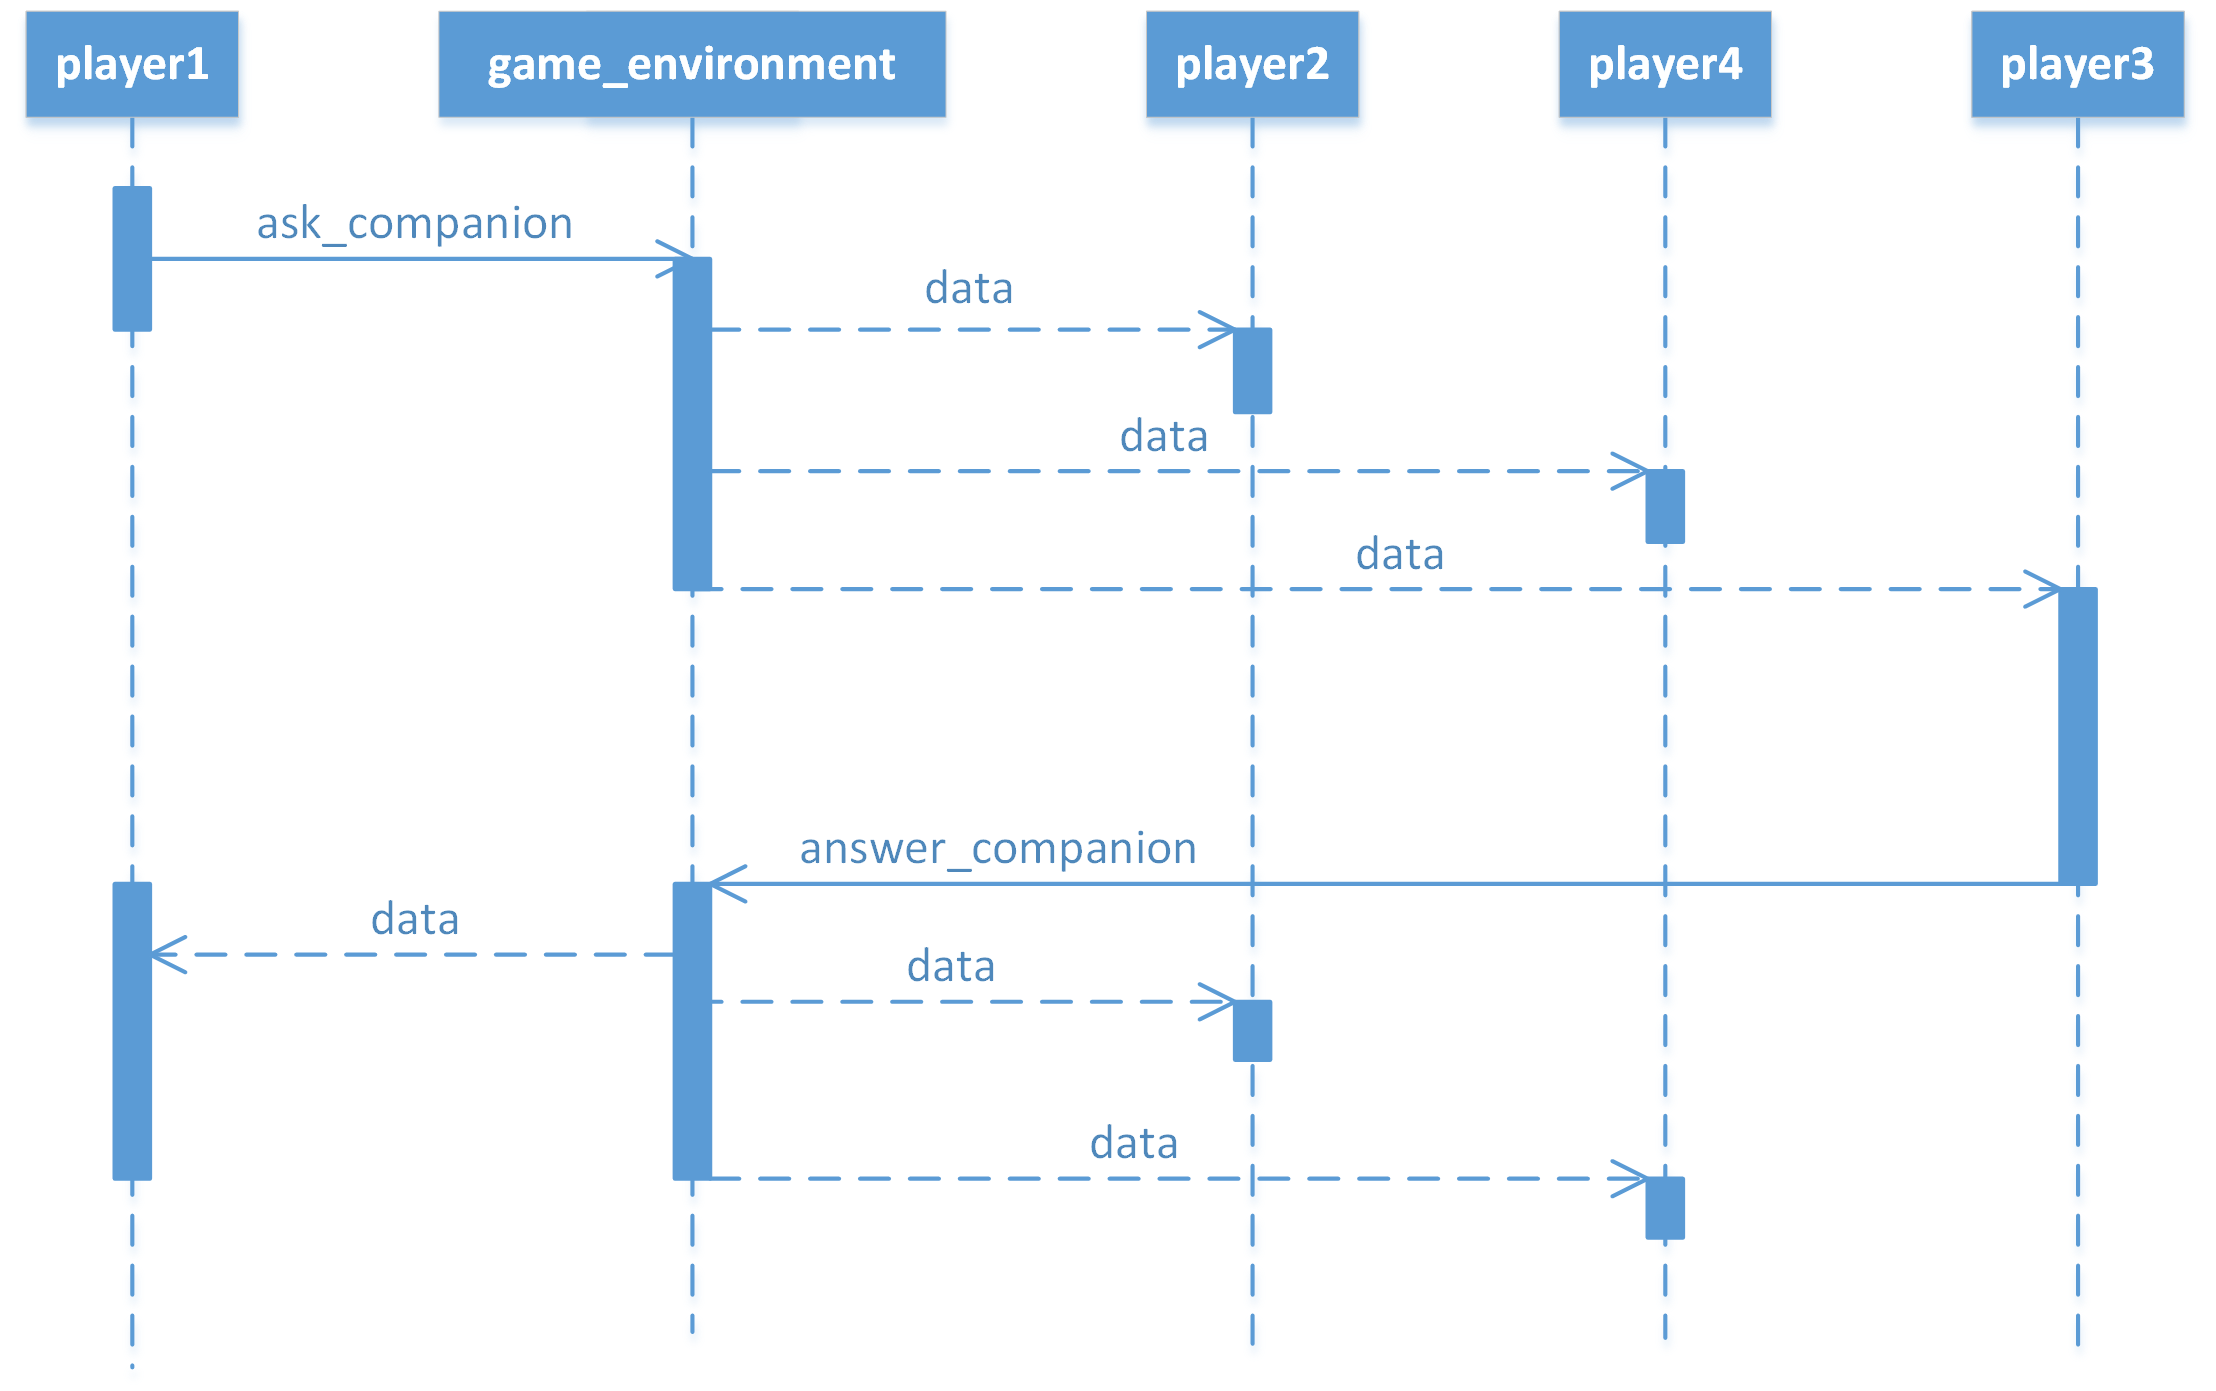
\includegraphics[width=180mm]{./img/speak_sequence_diagram.png}
	\caption{Diagramma di sequenza che mette in luce l'interazione tra i giocatori e il \emph{game environment}. \emph{Player1} è il giocatore di mano e avvia l'azione di parlare in modo da ricevere un'indicazione dal compagno \emph{player3}. Il \emph{game environment} media la comunicazione ed il flusso di informazioni che da esso giunge ai giocatori è rappresentato, con abuso di notazione, tramite delle frecce tratteggiate. \label{speak-sequence-diagram}}
\end{figure}


\section{Studio di fattibilità} \label{feasibility-study}
In questa sezione verranno anticipate ed analizzate le principali problematiche che potrebbero affliggere le successive fasi di sviluppo del sistema. Saranno inoltre proposte delle possibili soluzioni adottabili nella fase di progettazione. Nel sistema in esame l'unico aspetto che necessita di uno studio di fattibilità è quello relativo all'interazione tra i componenti.
\subsection{Interazione tra i componenti} \label{interactions}
Sono state individuate le principali modalità di interazione tra i componenti, analizzate di seguito.
\begin{description}
	\item[Scambio di messaggi]: dato che tutti i componenti sono stati definiti come entità attive, la scelta più immediata consiste in un approccio a scambio di messaggi. Questa tipologia di comunicazione è nativamente supportata dalle entità attive come attori e agenti, oltre che supportata dalla maggior parte dei linguaggi di comunicazione. Un ulteriore vantaggio è dato dal fatto che la comunicazione è diretta (senza mediatori), il che rende lo scambio di informazioni più veloce. Questo approccio, però, implica che ogni entità conosca il riferimento di tutte le entità con le quali vuole iniziare una comunicazione.
	\item[Pattern publish/subscribe]: rispetto allo scambio di messaggi, non vi è la necessità che il mittente conosca il riferimento del destinatario. Infatti, nella maggior parte dei casi, questo approccio mette a disposizione un \emph{broker} che funge da intermediario della comunicazione, garantendo scalabilità e disaccoppiamento tra i componenti, a costo di un \emph{delay} provocato dal broker stesso.
	\item[Spazio di tuple]: oltre alla memorizzazione dei dati, fornisce anche meccanismi avanzati per la coordinazione. Utilizzando uno spazio di tuple, non è più necessario che i componenti debbano essere reattivi alla ricezione di messaggi e alle notifiche emesse da un eventuale broker. Le entità, in questo modo, sono completamente proattive e decideranno di recuperare informazioni dallo spazio di tuple nel momento più opportuno.
\end{description}
Nel secondo e nel terzo approccio è prevista la presenza di un componente in grado di mediare la comunicazione (broker o spazio di tuple). Tale componente potrebbe essere una nuova entità (esterna al sistema attuale) o coincidere con il \emph{game environment}.

\section{Progettazione} \label{general-design}
In questa sezione verranno discusse le scelte progettuali effettuate e verrà proposta l'architettura generale del sistema.

\subsection{Scelte progettuali}
L'architettura del sistema sarà costruita prendendo come riferimento quanto proposto in \autoref{problem-analysis} e valutando i possibili approcci implementativi proposti in \autoref{feasibility-study}. I giocatori, il mazziere e l'arbitro sono sviluppati come agenti piuttosto che attori, in modo da porre l'enfasi sull'autonomia e la proattività di tali componenti.

Per la definizione dell'interazione dei componenti del sistema è scelto un approccio ibrido tra le tipologie proposte in \autoref{interactions}. Il \emph{game environment} è realizzato come uno spazio di tuple, sia per i vantaggi illustrati in precedenza, sia per il livello di astrazione che questo approccio presenta, che risulta essere vicino alla realtà. Ad esempio, in una partita reale una carta viene giocata appoggiandola sul tavolo e da quel momento risulta visibile a tutti i giocatori; allo stesso modo, una tupla inserita nello spazio di tuple può essere vista e consultata dagli agenti in ogni momento, fino a che non viene rimossa. Inoltre, l'azione di parlare risulta comodamente effettuabile attraverso uno spazio di tuple, semplicemente rappresentando domande e risposte come delle tuple, a cui tutti i giocatori possono accedere. Come diretta conseguenza di questa scelta, chiunque debba comunicare con il \emph{game environment} lo farà utilizzando le primitive fornite dal modello di coordinazione.

Tuttavia lo spazio di tuple non è la scelta migliore per alcuni scambi di informazioni tra i componenti. Le interazioni che non riguardano direttamente il \emph{game environment} potrebbero anch'esse essere mediate dallo spazio di tuple, oppure effettuate in maniera separata. Per salvaguardare l'integrità del modello e per attenersi il più possibile allo svolgimento reale di una partita del gioco, si decide di effettuare queste interazioni al di fuori dello spazio di tuple. Ad esempio, alcune comunicazioni non interessano direttamente i giocatori (come l'interazione fra arbitro e mazziere), mentre altre devono rimanere private ad un singolo giocatore (come la distribuzione delle carte). Per tutte queste interazioni si sceglie di adottare un approccio a scambio di messaggi, siccome ognuna di esse è finalizzata allo scambio di informazioni tra due sole entità.
L'architettura completa del sistema è illustrata in \autoref{general-architecture}.

\begin{figure}[H]
	\centering
	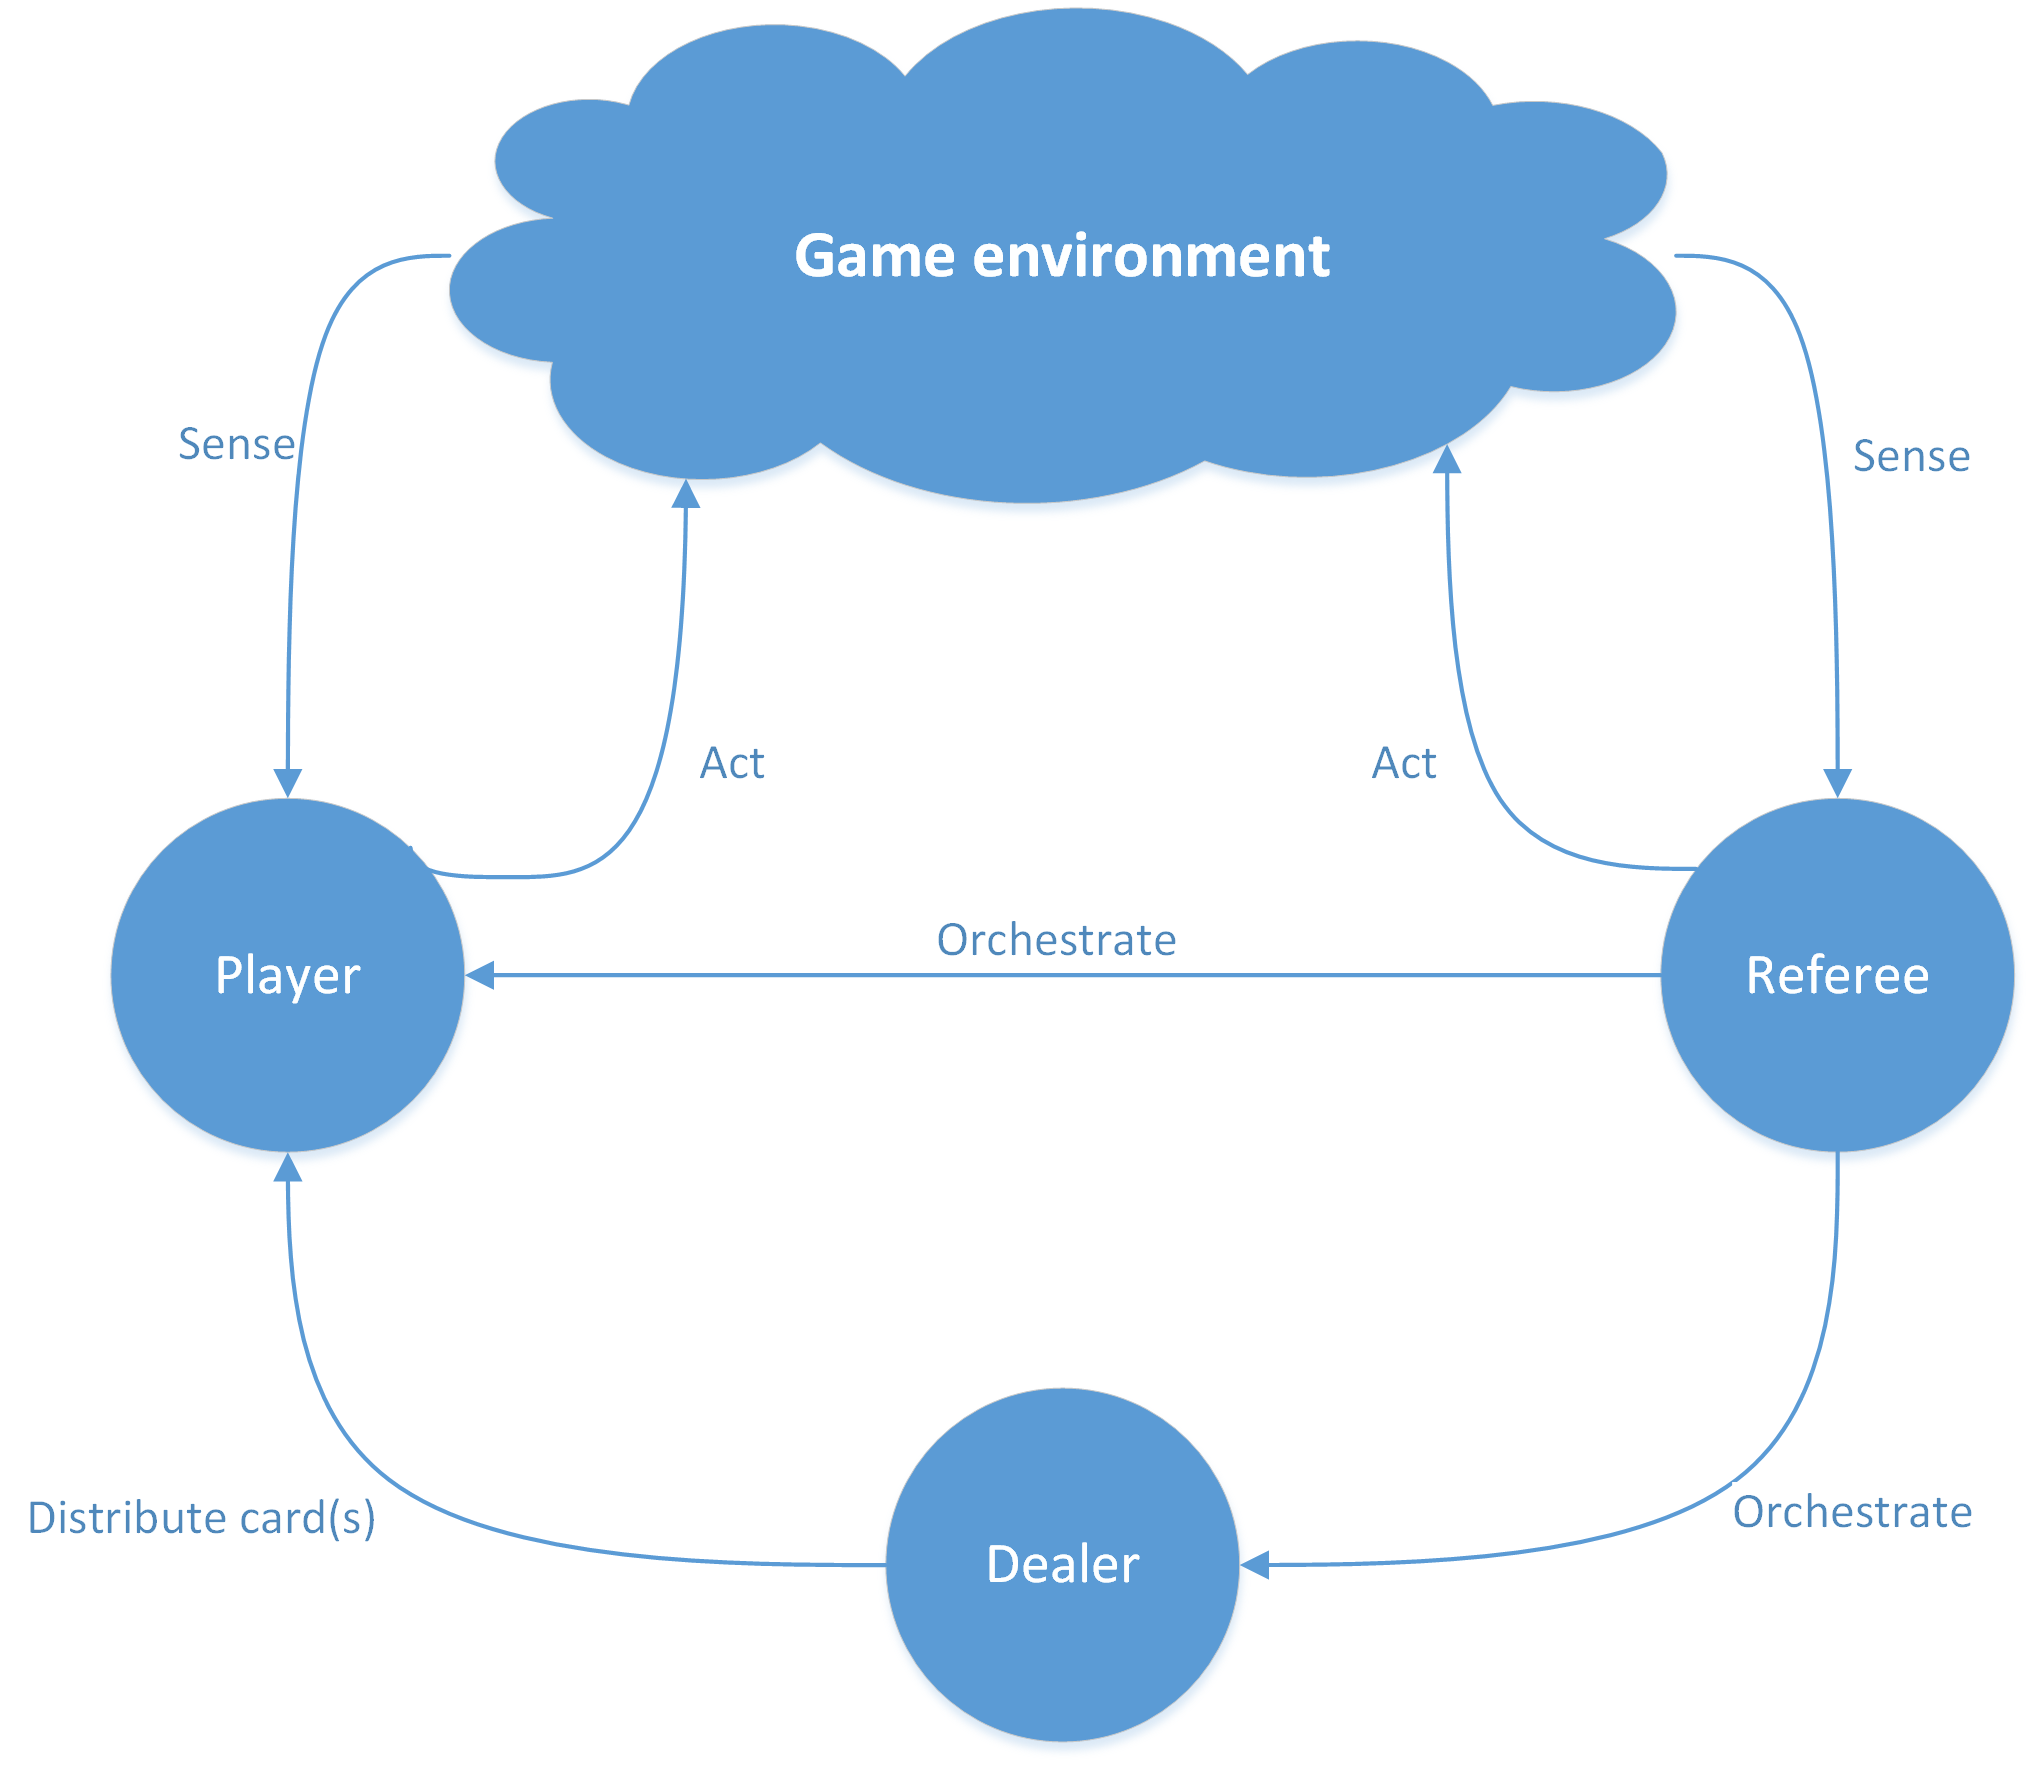
\includegraphics[width=\textwidth]{./img/general_architecture.png}
	\caption{Architettura generale del sistema. Per motivi di chiarezza grafica è rappresentato un solo giocatore. I giocatori interagiscono  con lo spazio di tuple attraverso le primitive \emph{out}, che consente di aggiungere una tupla all'interno dello spazio, e \emph{in}, che consente di interrogare il tuple space sulla presenza di una tupla e leggerla. Le interazioni tra agenti non mediate dal \emph{game environment} avvengono tramite scambio di messaggi.\label{general-architecture}}
\end{figure}


\subsection{Design di dettaglio} \label{design}

Fissati struttura del sistema ed interazione, si passa ora ad una fase di design di dettaglio, che prevede un raffinamento per quei componenti che presentano ancora alcune lacune per poter essere effettivamente implementati. 

Per quanto concerne arbitro e mazziere, non è necessario apportare perfezionamenti: essi dovranno semplicemente sottostare al regolamento di gioco attenendosi allo schema di interazione illustrato in \autoref{general-architecture}. Lo stesso discorso non può essere fatto per i giocatori, la cui logica interna utilizzata per scegliere la prossima carta da giocare non è ancora stata esplicitata. Si sceglie di assegnare ad ogni carta in mano una priorità, ovvero un valore che esprima quanto sia conveniente giocare una carta in relazione alle altre. Durante la fase di reasoning, questo valore può cambiare a seconda delle informazioni che il giocatore acquisisce, siano esse ricevute come risposta del compagno ad una domanda o acquisite mediante la consultazione delle carte già giocate sul tavolo. Più nello specifico, la valutazione di una carta avviene tramite tre fasi:
\begin{enumerate}
	\item \textbf{Assegnamento iniziale della priorità}: ad ogni carta viene assegnata una certa priorità sulla base del suo valore. In questa fase iniziale il giocatore assegna priorità più alta alle carte con valore più basso, in modo da giocare meno punti possibili qualora esso non riesca ad acquisire informazioni utili dal compagno o dal tavolo. Sempre per questa motivazione, alle briscole viene assegnata priorità bassa, di modo da conservarle per momenti più opportuni.
	\item \textbf{Valutazione delle carte sul tavolo}: il giocatore consulta le eventuali carte già giocate sul tavolo e modifica la priorità delle proprie carte sulla base della seguente strategia: se la dominante è la carta del compagno, allora aumenta la priorità di figure e carichi, di modo da giocare più punti possibile. Se invece la dominante è la carta di uno dei due avversari, il giocatore aumenta la priorità delle carte in grado di prendere sulla dominante stessa.
	\item \textbf{Domande al compagno}: qualora sia abilitato a farlo, in questa terza fase il giocatore di mano procede nel formulare una o più domande al compagno nel caso non abbia ancora certezza su quale carta giocare. L'ordine e la natura delle domande è stabilito dalla priorità attuale delle carte in mano: la prima sarà finalizzata ad acquisire informazioni utili a modificare la priorità della carta con priorità maggiore, procedendo poi con domande utili per le carte a priorità più bassa qualora sia necessario.    
\end{enumerate}

È importante precisare che a volte la valutazione potrebbe non passare per tutte le fasi illustrate. Ad esempio, se a seguire della prima fase il giocatore ha un certo livello di confidenza nel giocare una determinata carta rispetto alle altre (ovvero, la priorità della carta è maggiore di una soglia stabilita a priori), allora giocherà quella carta senza eseguire le successive fasi di valutazione. 

\section{Implementazione} \label{implementation}
In questa sezione verranno descritte le scelte fatte in fase di implementazione, basate sulla progettazione, descritta in \autoref{general-design}. I due componenti principali del progetto sono risultati il sistema multiagente e lo spazio di tuple; di seguito sono riportate, per ognuno di essi, le scelte implementative di maggior rilievo.  
\subsection{Agenti}
	Abbiamo scelto di utilizzare \emph{Jason}\footnote{\url{http://jason.sourceforge.net/wp}} per l'implementazione degli agenti. Esso è un interprete basato su \emph{Java} di una versione estesa del linguaggio \emph{AgentSpeak} con sintassi molto simile a quella del \emph{prolog}. Tramite tale linguaggio è possibile programmare i singoli agenti a livello di \emph{beliefe}, \emph{goal} e \emph{piani}. Ogni agente è stato implementato in modo indipendente, seguendo i compiti a lui assegnati in \autoref{design}. L'interazione tra gli agenti avviene come definito in \autoref{problem-analysis}, e si basa su scambio di messaggi o coordinazione tramite lo spazio di tuple. 
	
	Gli agenti non hanno solamente un comportamento proattivo, ma grazie all'infrastruttura messa a disposizione da \emph{Jason}, essi sono reattivi alla ricezione di messaggi. Infatti, ogni messaggio recapitato ad un agente, viene inserito nella sua base di conoscenza, come un semplice \emph{beliefe}. \`{E} possibile aggiungere un \emph{behaviour} alla base di conoscenza dell'agente, che viene eseguito ogni qualvolta un messaggio viene inserito al suo interno. Tale flusso di esecuzione è parallelo a quello principale dell'agente, e nel caso arrivino più messaggi saranno eseguiti più flussi paralleli. In questo modo un agente riesce a essere reattivo alla ricezione dei messaggi, in modo semplice e totalmente trasparente 
\subsection{Spazio di tuple}
Abbiamo deciso di utilizzare \emph{TuCSoN}\footnote{\url{http://apice.unibo.it/xwiki/bin/view/TuCSoN/WebHome}} come spazio di tuple. Purtroppo non è possibile utilizzare \emph{TuCSoN} nativamente all'interno di codice interpretato da \emph{Jason}, per cui ci siamo avvalsi della libreria \emph{TuCSoN4Jason}\footnote{\url{https://apice.unibo.it/xwiki/bin/view/TuCSoN/4Jason}}, che come \emph{TuCSoN} è stata sviluppata all'interno dell'Università di Bologna. 

In fase di implementazione è stato necessario creare un nuovo agente, chiamato \texttt{boot\_agent}, il quale ha lo scopo di inserire, all'avvio del sistema, le reazioni necessarie all'interno dello spazio di tuple. Tali reazioni sono: 
\begin{itemize}
	\item Unione delle tuple inerenti ad una domanda, e alla sua risposta, all'interno di un'unica tupla: \emph{conversation}.
	\item Rimozione dell'ultima mano giocata, una volta che l'arbitro ne inserisce una nuova.
	\item Inserimento, all'inizio della partita, della tupla vuota inerente all'ultima mano giocata (poiché nessuna mano è stata ancora giocata).
\end{itemize}
\section{Conclusioni} \label{conclusions}

\fancyhead{}
\renewcommand{\headrulewidth}{0pt}
\appendix
\addcontentsline{toc}{section}{Appendice}
\section*{Appendice}

\subsection*{Regole del gioco della briscola - 4 giocatori}\label{briscola-rules}

Non avendo trovato un regolamento ufficiale, si è preso come riferimento quello generale riportato in \footnote{\url{https://it.wikipedia.org/wiki/Briscola}}, con qualche piccola variazione.
 
I giocatori giocano in coppie di due, con un mazzo di 40 carte regionali. I punti disponibili per ogni partita sono in totale 120, vince chi ne realizza almeno 61; se i punti sono 60 per entrambe le coppie, la partita è pareggiata. I valori di presa sono nell'ordine decrescente: Asso, 3, Re, Cavallo, Donna o Fante, 7, 6, 5, 4 e 2. I giocatori devono essere disposti facendo sì che ognuno di essi abbia ai suoi lati i giocatori della squadra avversaria, in modo che due giocatori della stessa squadra non giochino mai consecutivamente. Disposti i giocatori, il mazziere mischia le carte senza guardare il mazzo, distribuisce 3 carte ciascuno e lascia una carta sul tavolo coprendola per metà con il mazzo posto trasversalmente ad essa, in modo che rimanga visibile a tutti per l'intero gioco: questa carta segnerà il seme di briscola e sarà l'ultima carta ad essere pescata. Partendo dal primo giocatore (quello che ha ricevuto la prima carta) e continuando in senso antiorario, ogni giocatore calerà la carta che riterrà più opportuna, con lo scopo di aggiudicarsi la mano o di totalizzare il maggior numero di punti assieme al proprio compagno. Da parte dei giocatori non esiste alcun obbligo di giocare un particolare tipo di seme. L'aggiudicazione della mano avviene secondo regole molto semplici:
\begin{itemize}
	\item il primo giocatore di mano determina il seme di mano calando la sua carta, detta dominante, e virtualmente è il vincitore temporaneo della mano.
	\item la mano può essere temporaneamente aggiudicata ad un altro giocatore se questi posa una carta del seme di mano con valore di presa maggiore (si dice che il giocatore ha "strozzato" la dominante), oppure giocando una qualsiasi carta del seme di briscola, anche con valore di presa inferiore rispetto alla carta dominante. Bisogna sottolineare che non vi è obbligo di risposta al seme della dominante.
\end{itemize}
Alla fine la mano è vinta dal giocatore che ha calato la carta di briscola col valore di presa maggiore o, in mancanza di questa, dal giocatore che ha calato la carta del seme di mano con il valore di presa maggiore. Se nessuno ha strozzato la dominante e se nessuno ha giocato una briscola, la mano è vinta dal primo giocatore di mano. Il giocatore che vince la mano prende tutte le carte poste sul tavolo e le ripone coperte davanti a sé; in seguito sarà il primo a prendere la prima carta dal mazziere, seguito da tutti gli altri sempre in senso antiorario e sarà il primo ad aprire la mano successiva e quindi a decidere il nuovo seme di mano. Alla prima mano è vietato parlare, diversamente dal resto della partita dove si può parlare. Quando il mazziere esaurisce le carte, i giocatori continuano a giocare fino ad esaurire le carte che hanno in mano. A quel punto la partita termina e si procede al conteggio dei punti (in una partita a 4 giocatori, una partita termina dopo 10 mani di gioco). Il punteggio di una squadra è dato dalla somma dei punti dei due giocatori che ne fanno parte. I punteggi delle carte sono riportate di seguito:

\begin{center}
	\begin{tabular}{| l | l | l | l | l | l | l |}
		\hline
		\textbf{Carte} & Asso & 3 & Re & Cavallo & Fante & 7-2 \\ \hline
		\textbf{Punti} & 11 & 10 & 4 & 3 & 2 & 0 \\ 
		\hline
	\end{tabular}
\end{center}

Durante lo svolgimento della partita, alle squadre non è consentito consultare le proprie prese dei turni precedenti per conteggiare i punti guadagnati. Tuttavia, in ogni momento, entrambe le squadre hanno diritto a consultare l'ultima presa che è stata fatta, ovvero quella della mano precedente.

\end{document}
